\documentclass[12pt, oneside]{book}
\usepackage[a4paper,top=2.5cm,bottom=2.5cm,left=3.5cm,right=2cm]{geometry}
\usepackage[utf8]{inputenc}
\usepackage[T1]{fontenc}
\usepackage{graphicx}
\usepackage{url}
\usepackage{listings}
\usepackage{amsmath}
\usepackage[hidelinks,breaklinks]{hyperref}
\usepackage{amssymb}
\usepackage{amsthm}
\usepackage{floatrow}
\usepackage{float}
\usepackage[english]{babel}
\usepackage[final]{pdfpages}
\usepackage{afterpage}
\usepackage[superscript,biblabel]{cite}

\newcommand\blankpage{%
    \null
    \thispagestyle{empty}%
    \addtocounter{page}{-1}%
    \newpage}
 
\theoremstyle{definition}
\newtheorem{definition}{Definition}[section]

\newcommand{\R}{\mathbb{R}}

\newcommand{\N}{\mathbb{N}}

\newfloatcommand{capbtabbox}{table}[][\FBwidth]

\DeclareMathOperator{\argmax}{arg\,max} % thin space, limits underneath in displays
%\usepackage[slovak]{babel} % vypnite pre prace v anglictine
\linespread{1.25} % hodnota 1.25 by mala zodpovedat 1.5 riadkovaniu

% -------------------
% --- Definicia zakladnych pojmov
% --- Vyplnte podla vasho zadania
% -------------------
\def\mfrok{2020}
\def\mfnazov{Hybrid genome assembly}
\def\mftyp{Magisterská práca}
\def\mfautor{Matúš Zeleňák}
\def\mfskolitel{Mgr. Tomáš Vinař PhD.}


\def\mfmiesto{Bratislava, \mfrok}

%aj cislo odboru je povinne a je podla studijneho odboru autora prace
\def\mfodbor{2508 Informatika} 
\def\program{ Informatika }
\def\mfpracovisko{ Katedra informatiky }

\begin{document}     
\frontmatter


% -------------------
% --- Obalka ------
% -------------------
\thispagestyle{empty}

\begin{center}
\sc\large
Univerzita Komenského v Bratislave\\
Fakulta matematiky, fyziky a informatiky

\vfill

{\LARGE\mfnazov}\\
\mftyp
\end{center}

\vfill

{\sc\large 
\noindent \mfrok\\
\mfautor
}

\eject % EOP i
% --- koniec obalky ----

% -------------------
% --- Titulný list
% -------------------
\thispagestyle{empty}
\noindent

\begin{center}
\sc  
\large
Univerzita Komenského v Bratislave\\
Fakulta matematiky, fyziky a informatiky

\vfill

{\LARGE\mfnazov}\\
\mftyp
\end{center}

\vfill

\noindent
\begin{tabular}{ll}
Študijný program: & \program \\
Študijný odbor: & \mfodbor \\
Školiace pracovisko: & \mfpracovisko \\
Školiteľ: & \mfskolitel \\
% Konzultant: & \mfkonzultant \\
\end{tabular}

\vfill


\noindent \mfmiesto\\
\mfautor

\eject % EOP i


% --- Koniec titulnej strany


% -------------------
% --- Zadanie z AIS
% -------------------
% v tlačenej verzii s podpismi zainteresovaných osôb.
% v elektronickej verzii sa zverejňuje zadanie bez podpisov

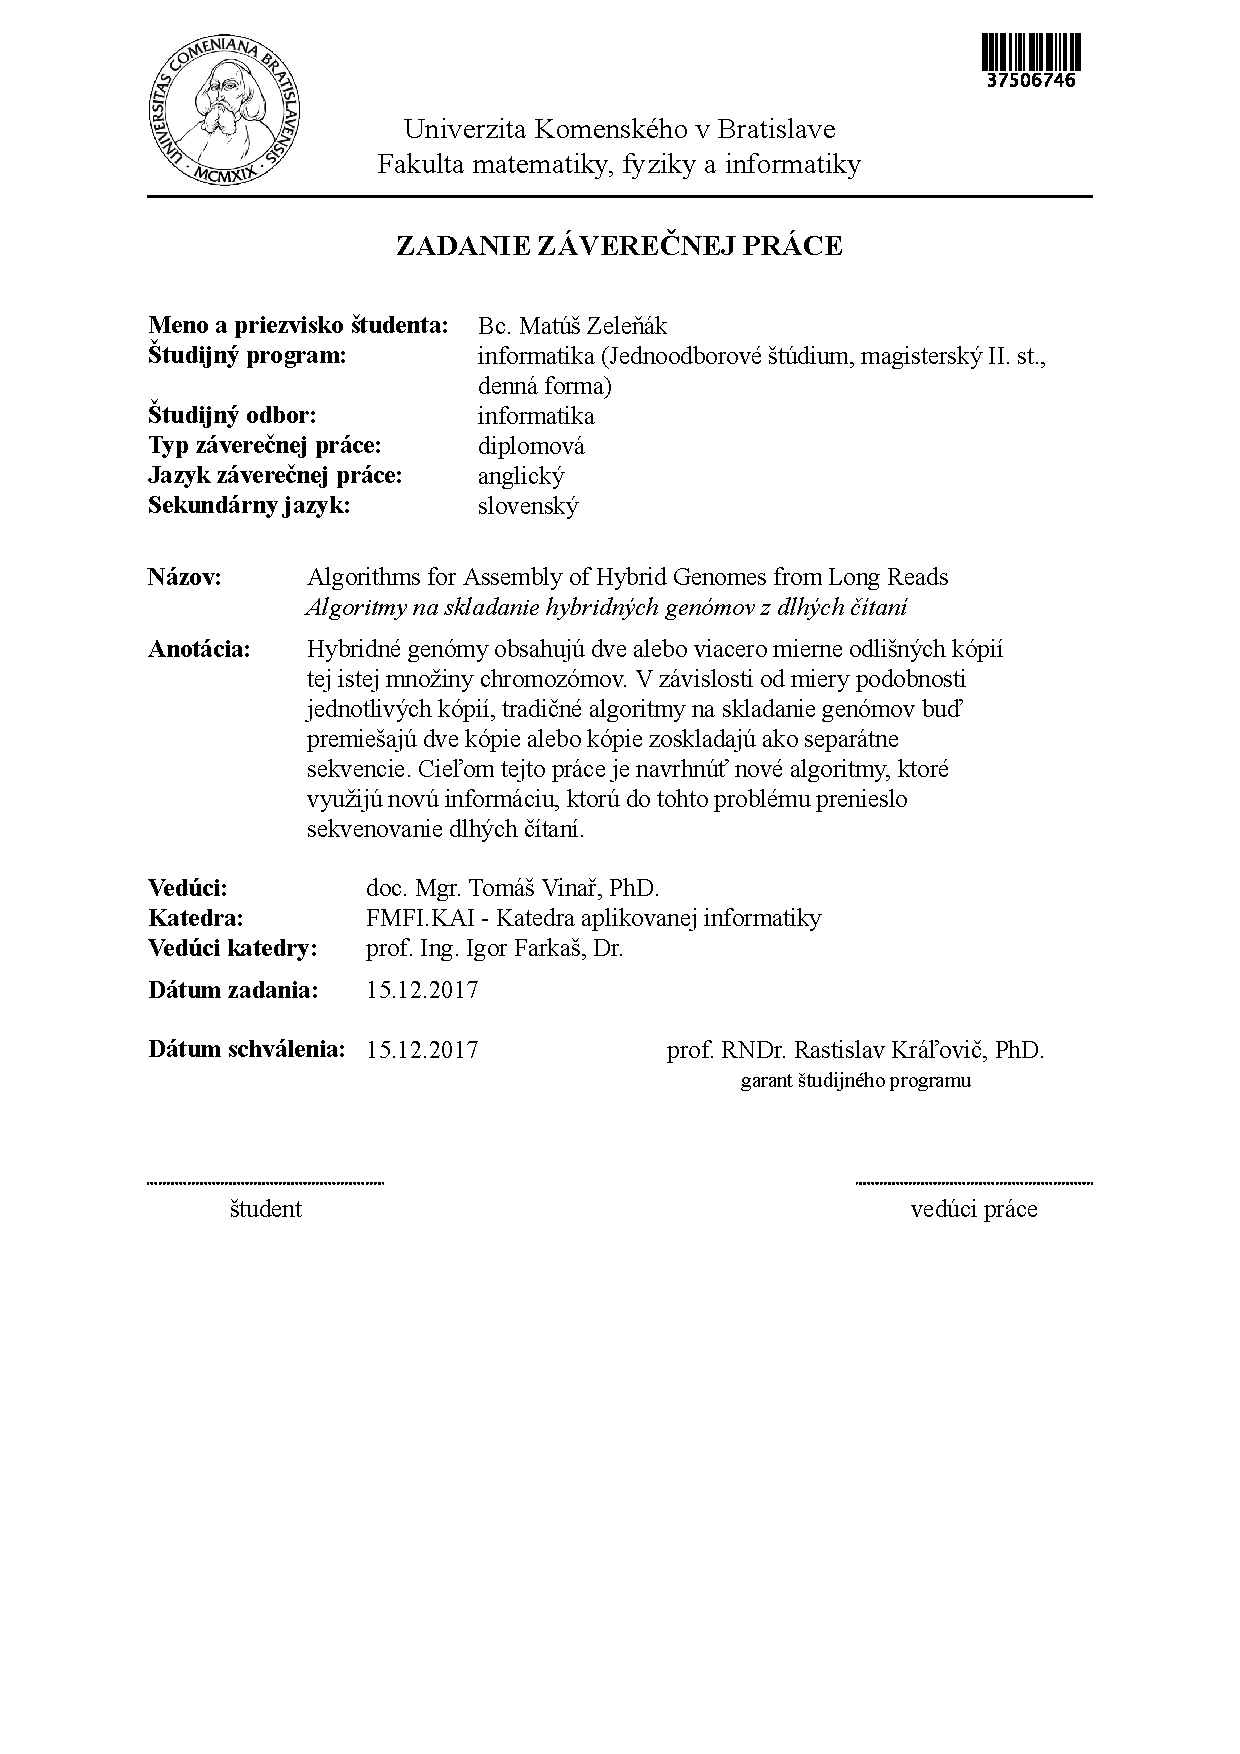
\includepdf[]{Assignment.PDF}

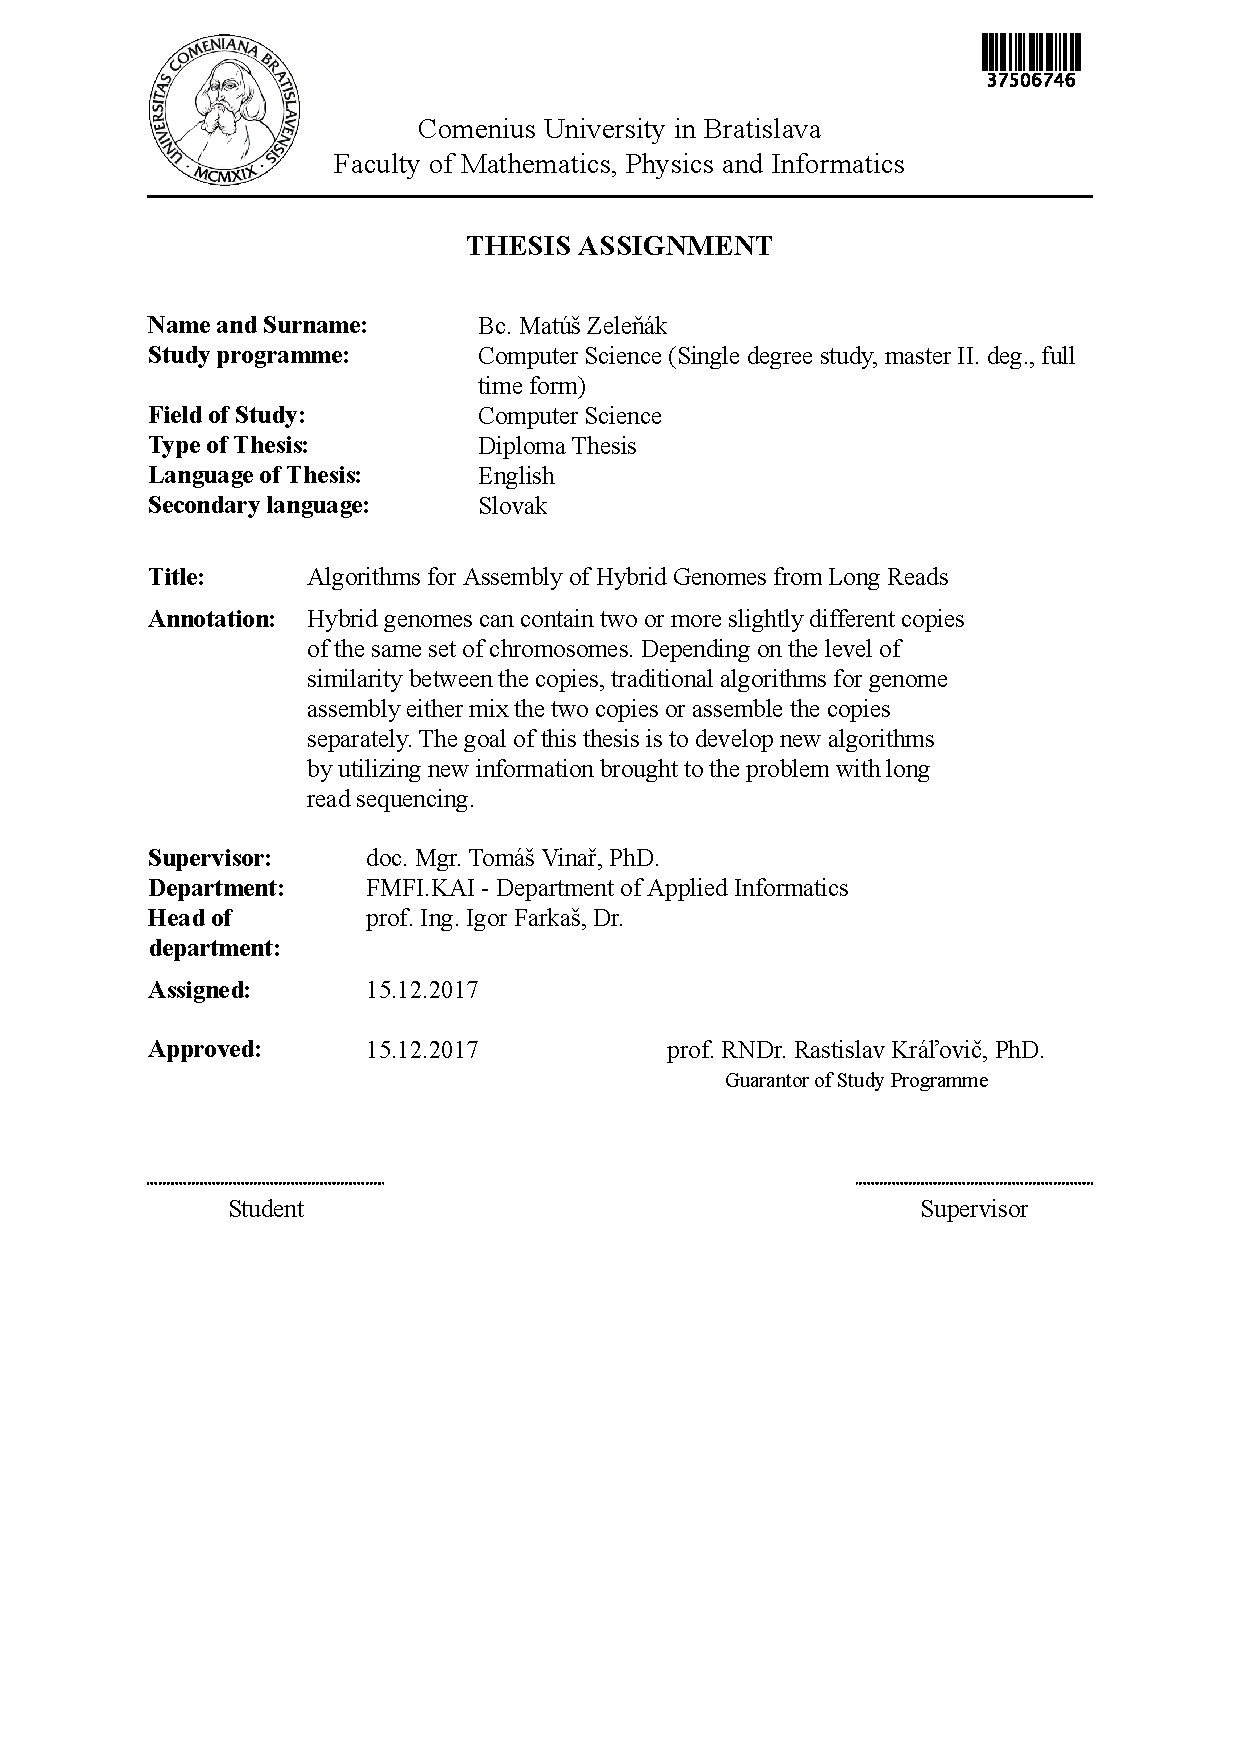
\includepdf[]{AssignmentEng.PDF}

%\hspace{-2cm}
%\includegraphics[width=1.1\textwidth]{images/zadanie}

% --- Koniec zadania

\frontmatter

% -------------------
%   Poďakovanie - nepovinné
% -------------------
\setcounter{page}{3}
~

\vfill
{\bf Acknowledgement:} I would like to thank Tomáš Vinař and Broňa Brejová for their guidance and patience and to Gareth Cooker for creating wonderful soundtracks that would carry me through the feverish nights of coding.

% --- Koniec poďakovania

% -------------------
%   Abstrakt - Slovensky
% -------------------
\newpage 
\section*{Abstrakt}

Hybridné genómy predstavujú výzvu pri skladaní haplotypov organizmov, keďže klasické 
nástroje na skladanie buď kópie chromozómov premiešajú do jednej sekvencie, alebo oddelia úplne.
V našej práci pristupujeme ku problému kategorizácie čítaní podľa ich príslušnosti k hybridu ako ku grafovému problému. Na základe špecifických $k$-tic zostrojíme spojenia medzi čítaniami a následne vytvárame čoraz väčšie komponenty, pričom sa snažíme zachovať nízku mieru medzihybridnej kontaminácie. Naše výsledky na zmiešaných simulovaných čítaniach dvoch kmeňov E.coli baktérie ukazujú, že kategorizácia čítaní diploidného genómu je v princípe možná s vysokou mierou presnosti a malými výpočtovými požiadavkami.	
Naše metódy aplikujeme na dosiaľ nepreskúmanú kvasinku Magnusiomyces spicifer a vyhodnotíme ako výsledky, tak aj možný budúci vývoj v oblasti skladania hybridných genómov.

\paragraph*{Kľúčové slová:} DNA, Haplotyp, kategorizácia, spektrálne zhlukovanie
% --- Koniec Abstrakt - Slovensky


% -------------------
% --- Abstrakt - Anglicky 
% -------------------
\newpage 
\section*{Abstract}

Hybrid genomes pose a challenge during read assembly of organism haplotypes, as standard assembly tools either mix the chromosome copies into one sequence, or separate the copies entirely.
In our work we approach the problem of categorizing reads according to their origin hybrid as a graph clustering problem, using specific $k$-mers to construct connections between the reads and subsequently creating incrementally larger components while trying to maintain low cross-hybrid read contamination. Our results on mixed simulated reads from different E.coli strains show that in principle categorization of diploid genomes is possible with high degree of accuracy and small computational cost. We apply our methods to a novel yeast strain Magnusiomyces spicifer and examine both the results and possible future direction of development in the area of hybrid genome assembly.

\paragraph*{Keywords:} DNA, Haplotype, categorization, spectral clustering

% --- Koniec Abstrakt - Anglicky


% -------------------
% --- Obsah
% -------------------

\newpage 

\tableofcontents

% ---  Koniec Obsahu

% -------------------
% --- Zoznamy tabuliek, obrázkov - nepovinne
% -------------------

\newpage 

\listoffigures
\listoftables

% ---  Koniec Zoznamov

\mainmatter

\input Introduction.tex

\input ProblemStatement.tex

\input Dataset.tex

\input DiscriminativeKmers.tex

\input Categorization.tex

\input Evaluation.txt

\input Implementation.tex

\input Conclusion.tex

% -------------------
% --- Bibliografia
% -------------------


\newpage	

\backmatter

\thispagestyle{empty}
\nocite{*}
\clearpage

\bibliographystyle{plain}
\bibliography{literatura} 

%---koniec Referencii

% -------------------
%--- Prilohy---
% -------------------

%Nepovinná časť prílohy obsahuje materiály, ktoré neboli zaradené priamo  do textu. Každá príloha sa začína na novej strane.
%Zoznam príloh je súčasťou obsahu.
%
% \addcontentsline{toc}{chapter}{Appendix A}
% \input AppendixA.tex


\end{document}





